The process that our experiment undertook was iterative. Obstacles in the analysis showed the need to develop tools that help us to make the process less cumbersome. In the same way that in the previous chapter we explored the flow of ideas that led to our pipeline design, here we will explain how data shaped our experimental process.\\

To have a complete picture of how does our approach compares with techniques from classical computer vision, we trained other models to test their performance against our novel approach.\\

\section{Exploratory analysis}

Drone images from three different towns in the state of Oaxaca where obtained from CENAPRED. During the week following the Chiapas earthquake of September 7, 2018, several drones took these pictures. We received 727 images from Santa Maria Xadani, 1872 from Union Hidalgo, and 1134 from Juchitan de Zaragoza.\\

\begin{figure}[!ht]
  \centering
    \begin{subfigure}{.8\textwidth}
        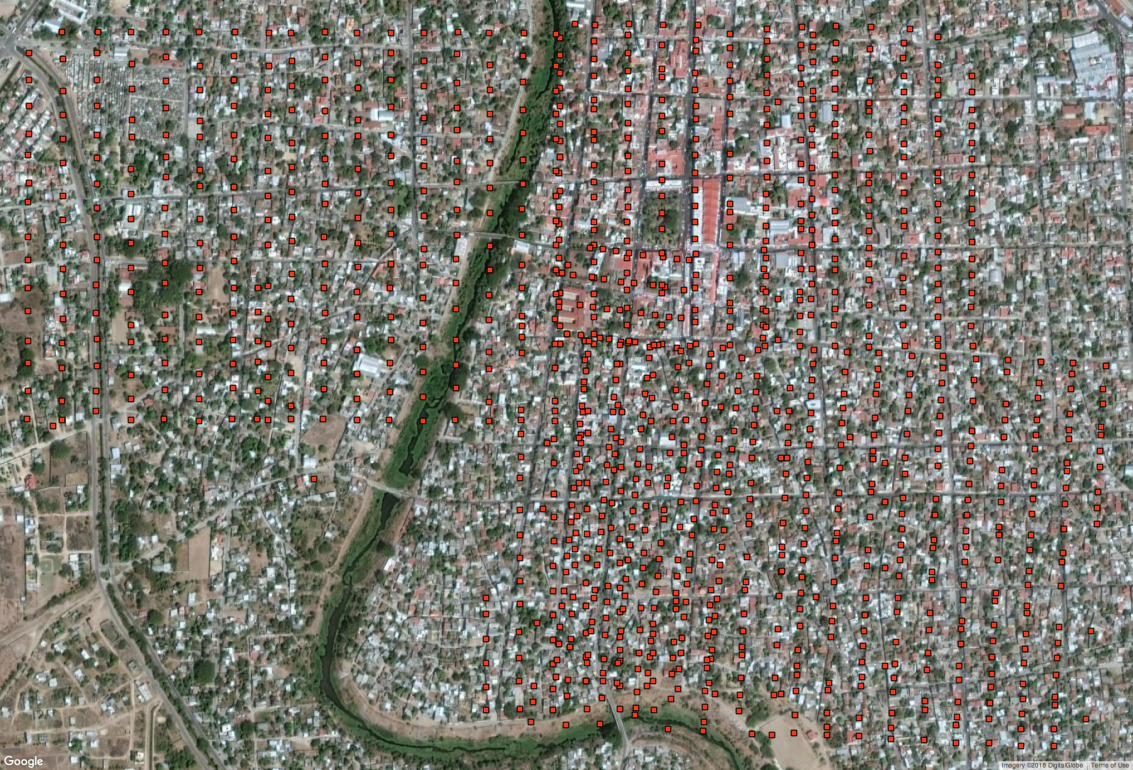
\includegraphics[width=\textwidth]{images/juchitan-satellite.jpg}
    \end{subfigure}
    \begin{subfigure}{.8\textwidth}
        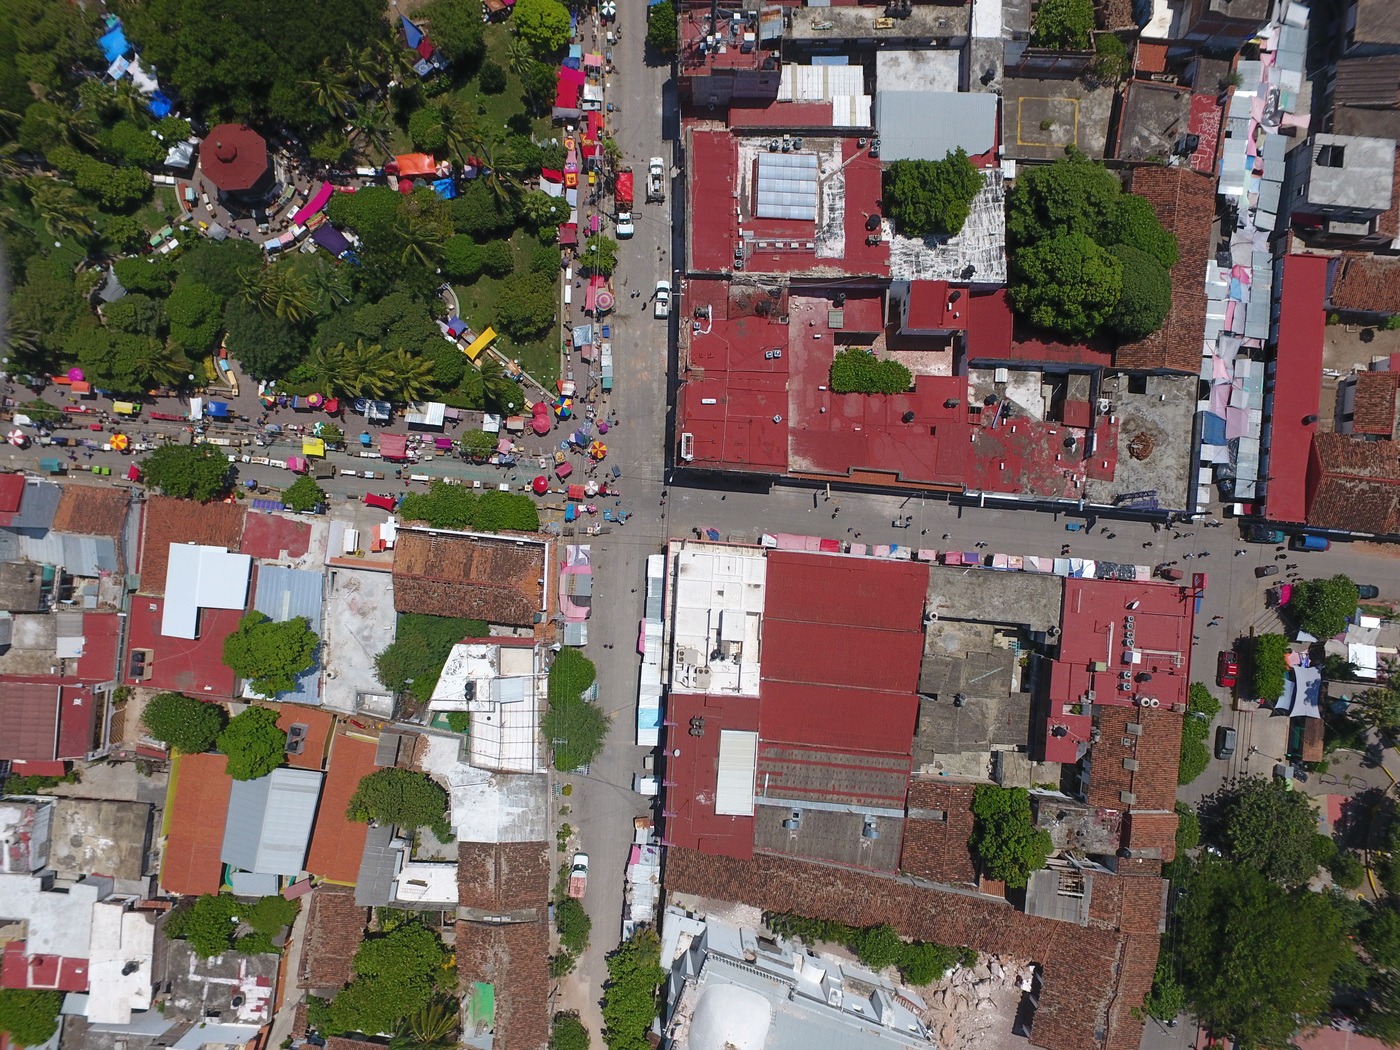
\includegraphics[width=\textwidth]{images/juchitan-sample.jpg}
    \end{subfigure}
  \caption{Juchit\'an de Zaragoza.}
  \label{fig:juchitan}
\end{figure}

\begin{figure}[!ht]
  \centering
    \begin{subfigure}{.8\textwidth}
        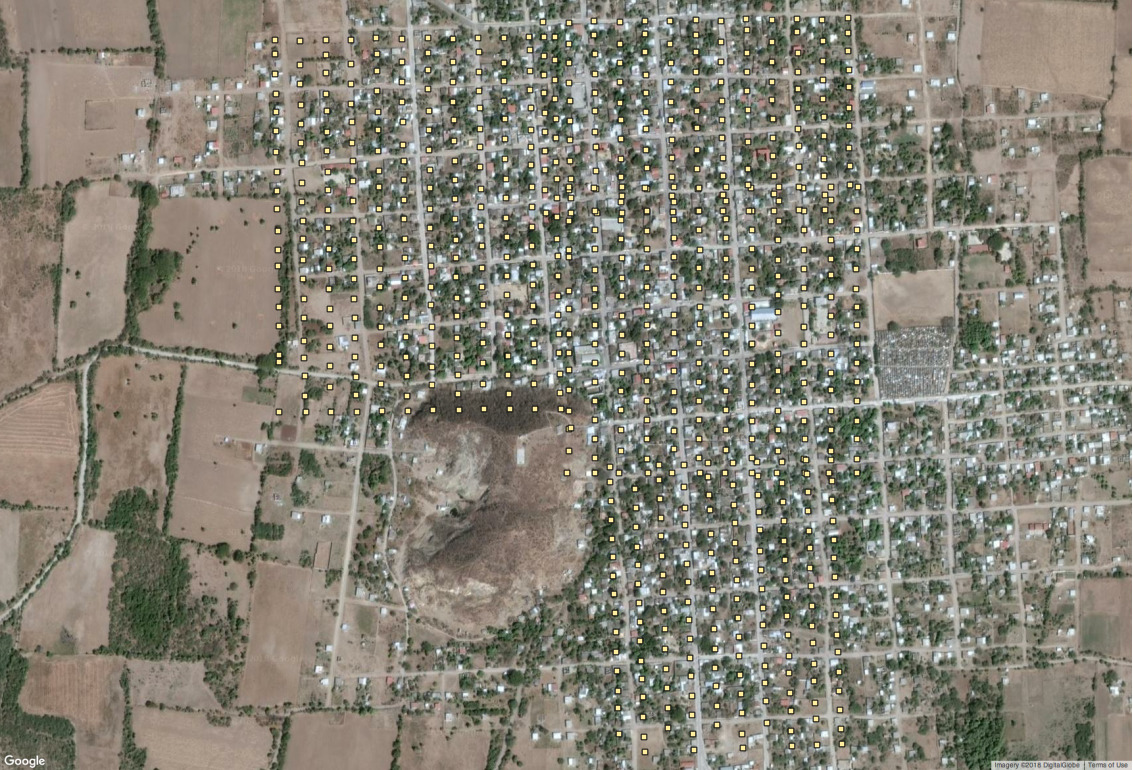
\includegraphics[width=\textwidth]{images/santamaria-satellite.jpg}
    \end{subfigure}
    \begin{subfigure}{.8\textwidth}
        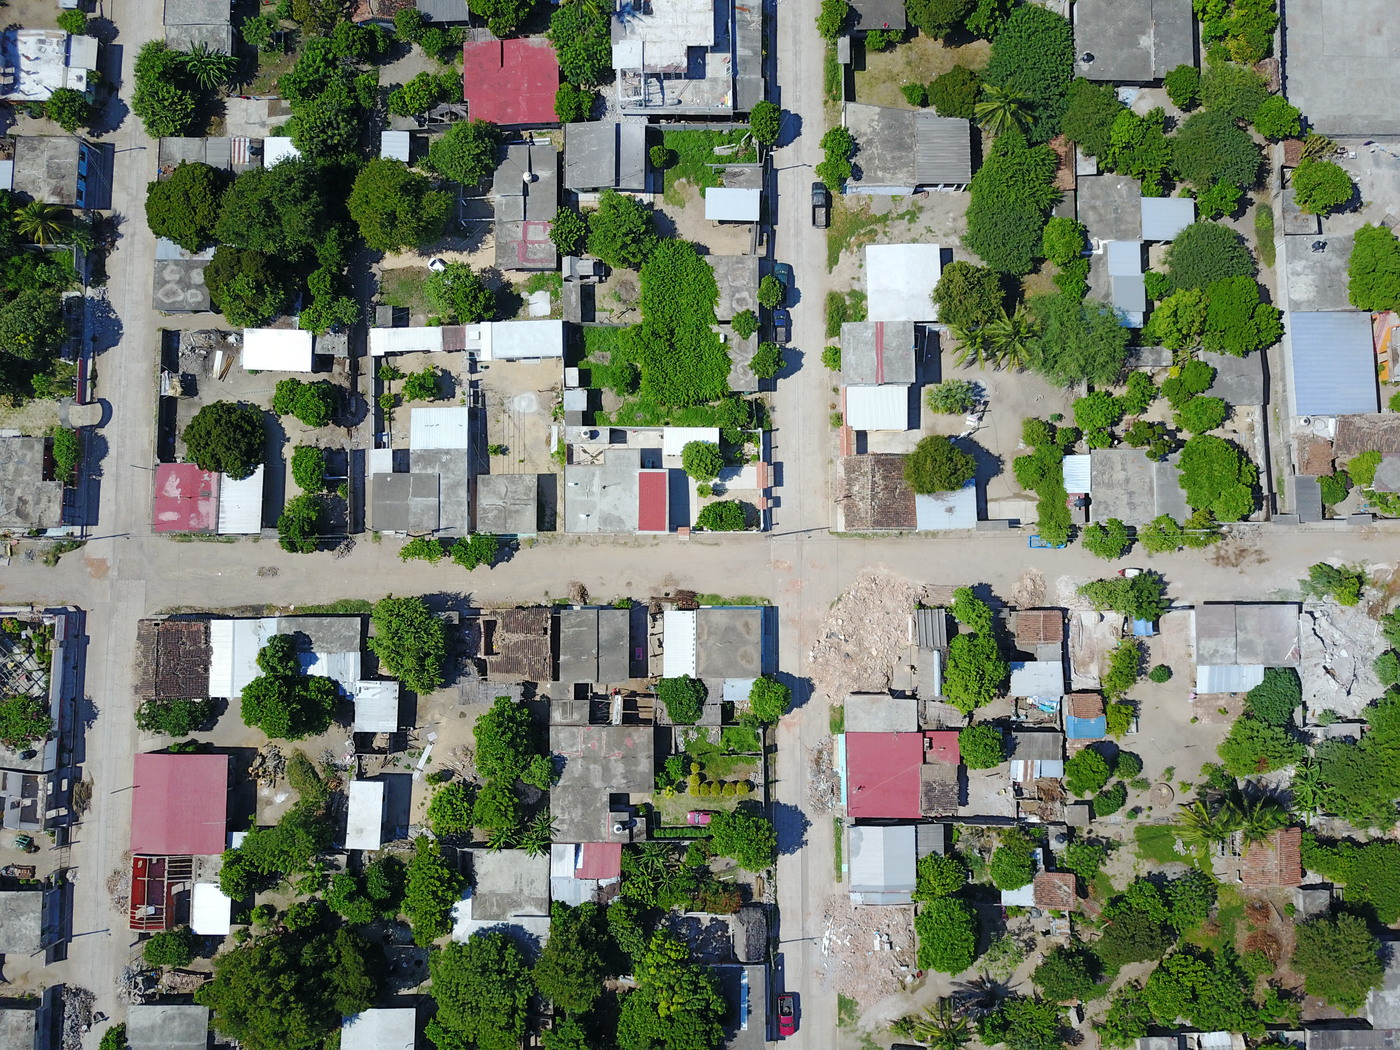
\includegraphics[width=\textwidth]{images/santamaria-sample.jpg}
    \end{subfigure}
  \caption{Santa Mar\'ia Xadani.}
  \label{fig:santamaria}
\end{figure}

\begin{figure}[!ht]
  \centering
    \begin{subfigure}{.8\textwidth}
        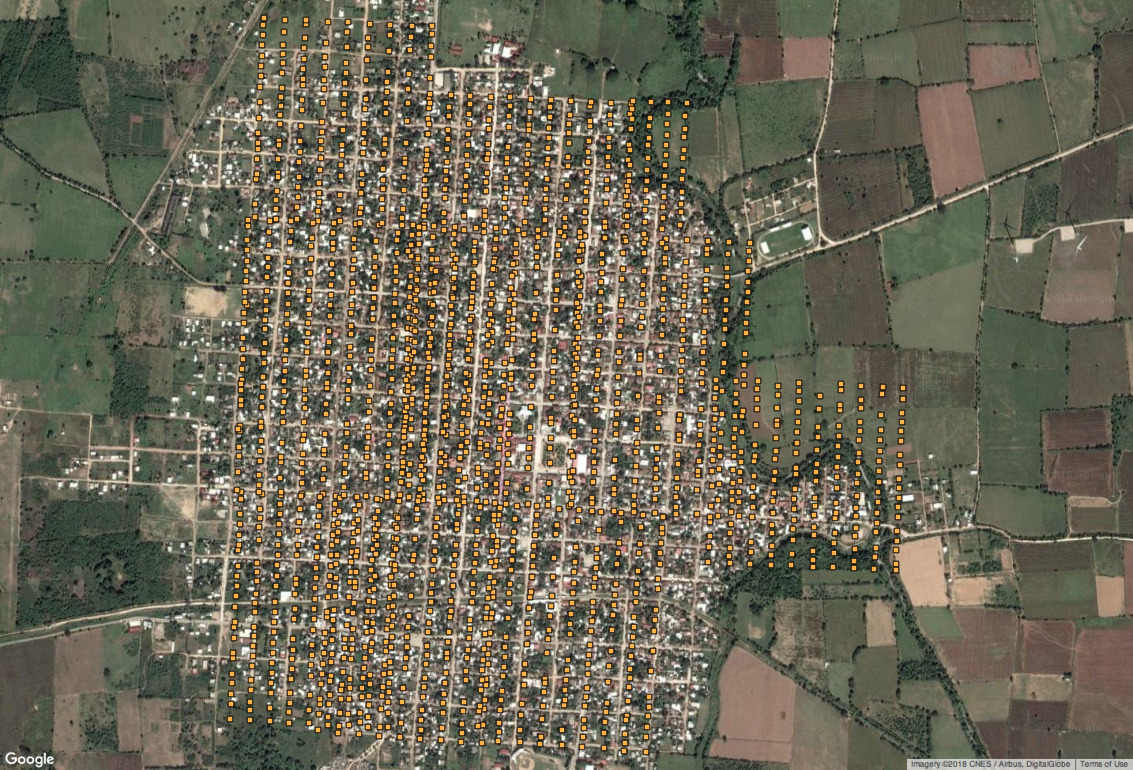
\includegraphics[width=\textwidth]{images/union-satellite.jpg}
    \end{subfigure}
    \begin{subfigure}{.8\textwidth}
        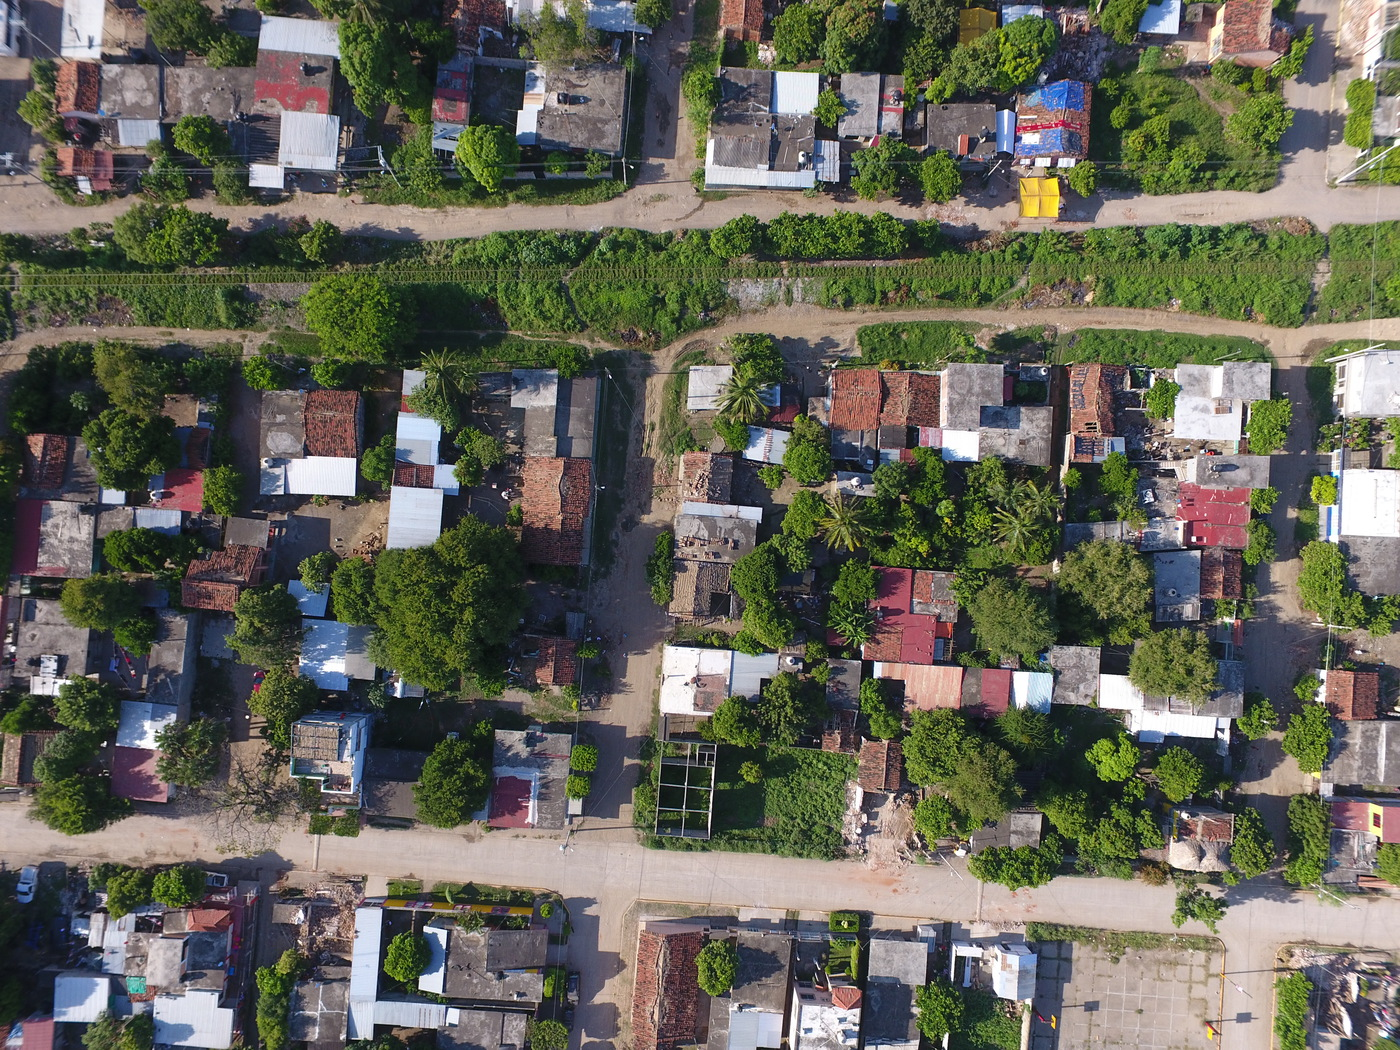
\includegraphics[width=\textwidth]{images/union-sample.jpg}
    \end{subfigure}
  \caption{Uni\'on Hidalgo.}
  \label{fig:union}
\end{figure}

As we can see in the Figures \ref{fig:juchitan}, \ref{fig:santamaria}, and \ref{fig:union}, drones fly in regular patterns forming a lattice of points. It is natural to think that given the spatial distribution, that the images distribute among similar clusters. First, we wanted to show that this clustering translates to the space of information that the images contain. To do this, we used a technique for our set of pictures known as t-distributed stochastic neighbor embedding. It was first introduced by Laurens van der Maaten \cite{t-sne}, as an alternative to traditional methods that were difficult to optimize.\\

In the interest of being able to represent the images in a two-dimensional structure, we used a technique known as t-distributed stochastic neighbor embedding (t-SNE) analysis. It usually captures the underlying structure of a set in a high dimensional space, and it is useful when the data lies in different, but low dimensional manifolds.\\

In our case we expected the images of the different towns to cluster in this low dimensional representation. We thought that pictures taken under in the same town would be closer than the ones taken in a different setting because of the light conditions during the exposure tend to have less variance among similar times and places. To this end, the information from the pixels of each image was flattened into a vector comprising the means and standard deviations. This simple dimensionality reduction technique was used to embed the images into a lower dimensional space using the aforementioned technique. As we expected, images form natural clusters depending on the town that they depict. Our result is shown in Figure \ref{fig:tsne}.\\

\begin{figure}[h]
  \centering
  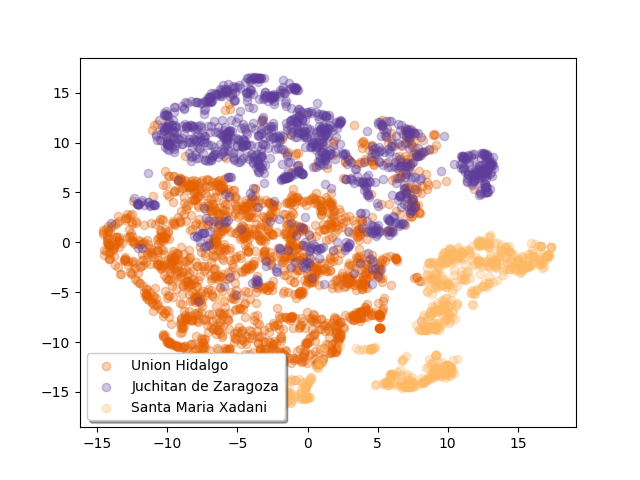
\includegraphics[width=1\textwidth]{images/t-sne.png}
  \caption{T-sne diagram.}
  \label{fig:tsne}
\end{figure}

The outcome obtained after applying t-SNE adds to evidence that supports our proposed methodology of using images from one town and try to predict on others.\\

We used the application detailed in the previous chapter to crop and classify 100 square patches from the images in each of the towns. Each piece was 327 x 327 pixels, and a tag was assigned manually for each of them. The information was stored in the relational database and reviewed for data consistency.\\

\begin{figure}[!ht]
  \centering
    \begin{subfigure}{.24\textwidth}
        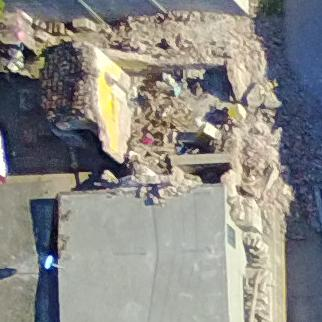
\includegraphics[width=\textwidth]{images/damaged1.jpg}
    \end{subfigure}
    \begin{subfigure}{.24\textwidth}
        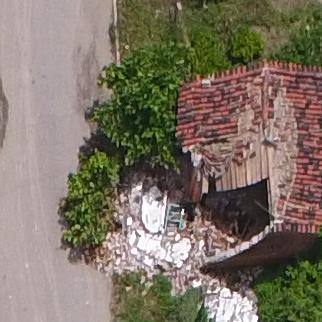
\includegraphics[width=\textwidth]{images/damaged2.jpg}
    \end{subfigure}
    \begin{subfigure}{.24\textwidth}
        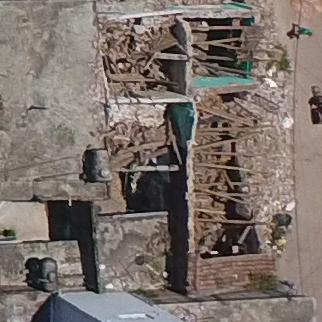
\includegraphics[width=\textwidth]{images/damaged3.jpg}
    \end{subfigure}
    \begin{subfigure}{.24\textwidth}
        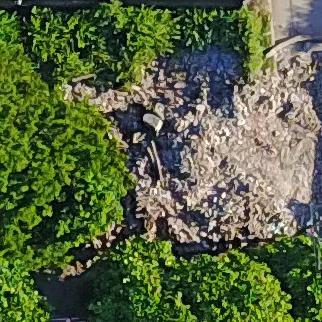
\includegraphics[width=\textwidth]{images/damaged4.jpg}
    \end{subfigure}
    %
    \begin{subfigure}{.24\textwidth}
        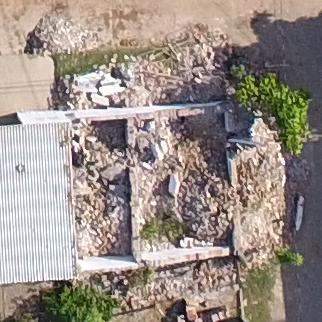
\includegraphics[width=\textwidth]{images/damaged5.jpg}
    \end{subfigure}
    \begin{subfigure}{.24\textwidth}
        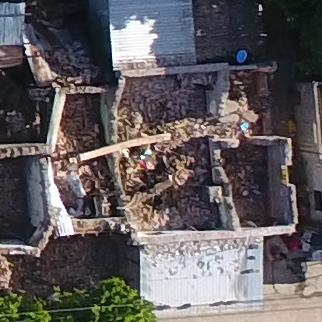
\includegraphics[width=\textwidth]{images/damaged6.jpg}
    \end{subfigure}
    \begin{subfigure}{.24\textwidth}
        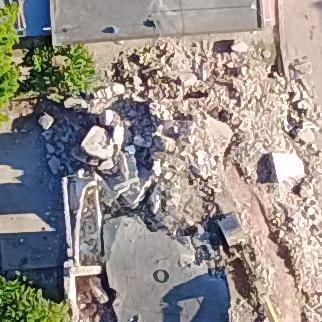
\includegraphics[width=\textwidth]{images/damaged7.jpg}
    \end{subfigure}
    \begin{subfigure}{.24\textwidth}
        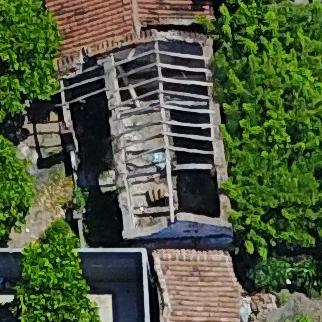
\includegraphics[width=\textwidth]{images/damaged8.jpg}
    \end{subfigure}
  \caption{Sample images from the damaged training set.}
  \label{fig:damaged}
\end{figure}


\begin{figure}[!ht]
  \centering
    \begin{subfigure}{.24\textwidth}
        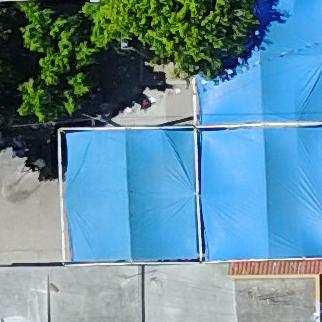
\includegraphics[width=\textwidth]{images/nondamaged1.jpg}
    \end{subfigure}
    \begin{subfigure}{.24\textwidth}
        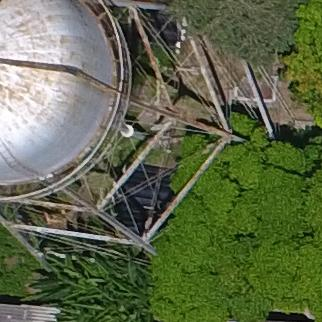
\includegraphics[width=\textwidth]{images/nondamaged2.jpg}
    \end{subfigure}
    \begin{subfigure}{.24\textwidth}
        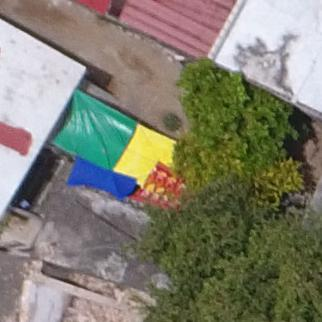
\includegraphics[width=\textwidth]{images/nondamaged3.jpg}
    \end{subfigure}
    \begin{subfigure}{.24\textwidth}
        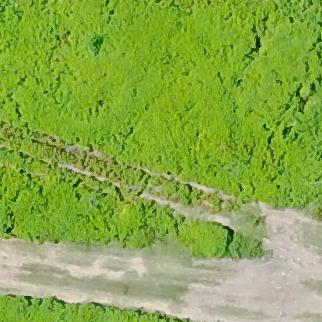
\includegraphics[width=\textwidth]{images/nondamaged4.jpg}
    \end{subfigure}
    %
    \begin{subfigure}{.24\textwidth}
        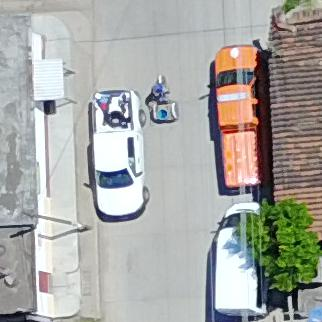
\includegraphics[width=\textwidth]{images/nondamaged5.jpg}
    \end{subfigure}
    \begin{subfigure}{.24\textwidth}
        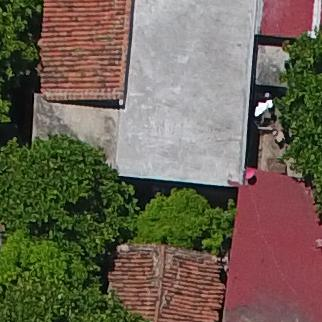
\includegraphics[width=\textwidth]{images/nondamaged6.jpg}
    \end{subfigure}
    \begin{subfigure}{.24\textwidth}
        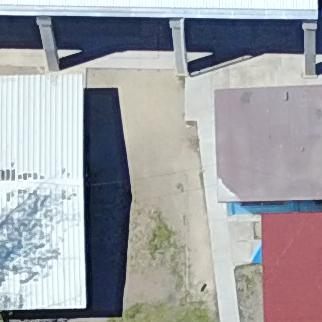
\includegraphics[width=\textwidth]{images/nondamaged7.jpg}
    \end{subfigure}
    \begin{subfigure}{.24\textwidth}
        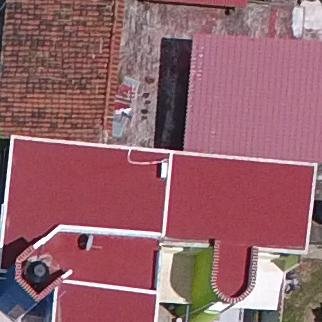
\includegraphics[width=\textwidth]{images/nondamaged8.jpg}
    \end{subfigure}
  \caption{Sample images from the non damaged training set.}
  \label{fig:nondamaged}
\end{figure}

To test the effectiveness of our method we need a benchmark for it. We decided to run an experiment with our data and classic computer vision methods. We extracted simple features from the images, and then we trained a classification model on the resulting data. By doing more complex feature engineering on the pictures, it would be likely to obtain better results. However, it was not the scope of the present work. We wanted to show how the methods compare out of the box with little extra effort.\\

We used three types of features. First, we use a method known as histogram oriented gradients (hog), introduced by William T. Freeman and Michal Roth \cite{MERL_TR94-03}. It consists of studying the slopes of the intensity of the pixels in a dense grid of the image. The feature space that this method output depends on the size of the lattice. Then, to test more straightforward features, and we extract the means and the standard deviations from each of the color channels. The result was a six-dimensional vector for each picture. We also decided to consider the means alone as a different training set. Finally, we trained a random forest for each of the resulting sets.\\

Our research targets a real environment in which data is scarcer. We are interested in the number of images needed to obtain good results. To research on that topic, we trained models feeding them with different training set sizes and testing them against a set of a fixed size. In summary, we trained a model for each combination of a method, a training set size, and a town permutation.\\

\section{Experiment}

In this secction we will explain the details about our results. As we mentioned before we study three different towns, we assembled different train, validate and test sets using different permutations each time. In the case of the classic computer vision methods, two towns were used to train and the remaining one was used to test the trained model. In the case of the transfer learning model, we use the images of one town to retrain the model, the images of another town to validate the model during the training stage, and the remaining town to test the trained model. In all cases every single image in the testing town was tested against the model.

\subsection{Classic Computer Vision}

We extracted the hog features using an implementation from the Python package scikit-image \cite{scikit-learn}. We used 8 orientations, and a $16\times16$ pixel window. Each town was selected once for testing, in table \ref{table:classic}, we assing labels that are later used in Figure \ref{fig:classic} to show the results that we obtained.


\begin{center}
  \begin{tabular}{|c|c|c|}
    \hline
    Train Set                                      &Test Set               &Code \\ \hline
    Juchit\'an de Zaragoza, Uni\'on Hidalgo        &Santa Mar\'ia Xadani   &JU-S \\ \hline
    Juchit\'an de Zaragoza, Santa Mar\'ia Xadani   &Uni\'on Hidalgo        &JS-U \\ \hline
    Santa Mar\'ia Xadani, Uni\'on Hidalgo          &Juchit\'an de Zaragoza &SU-J \\ 
    \hline
  \end{tabular}
  \label{table:classic}
\end{center}

\begin{figure}[ht]
  \centering
    \begin{subfigure}{.49\textwidth}
        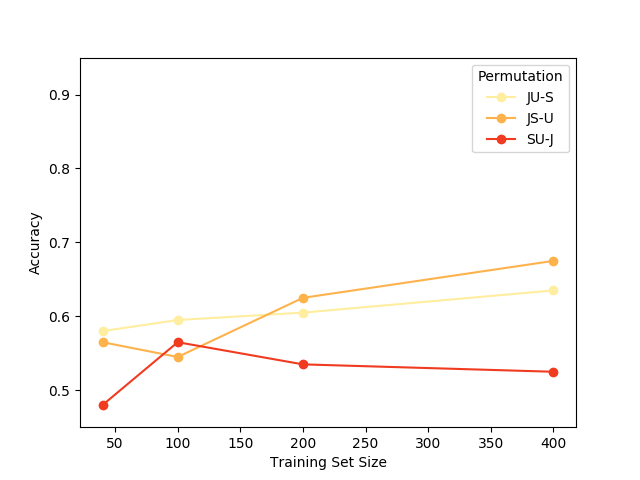
\includegraphics[width=\textwidth]{images/classic-hog.png}
        \caption{Histogram Oriented Gradients}
    \end{subfigure}
    \begin{subfigure}{.49\textwidth}
        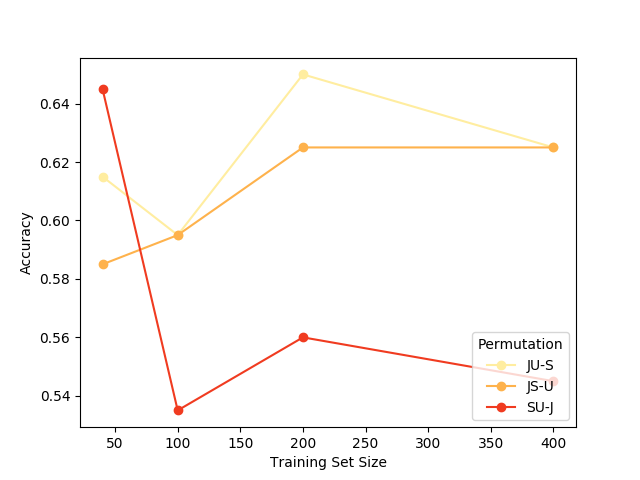
\includegraphics[width=\textwidth]{images/classic-means.png}
        \caption{Means}
    \end{subfigure}
    %
    \begin{subfigure}{.49\textwidth}
        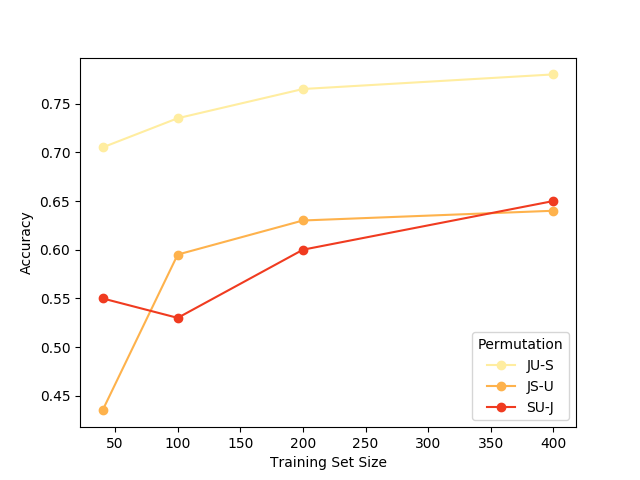
\includegraphics[width=\textwidth]{images/classic-meanstd.png}
        \caption{Means + Standard Deviation}
    \end{subfigure}
  
  \caption{Training example using classic computer vision models.}
  \label{fig:classic}
\end{figure}

It was surprising that the model that showed the best performance was the one in which we considered means and standard deviations. We expected that the specialized features from the HOG model performed better that a simple mean and standard deviation extraction. We think that this was because the HOG features were designed to find objects in images, but they are not well suited for aerial images and the textures that characterizes the ribble. As we expected increasing the size of the training set results in improving the performance of the trained model. In particular we noticed that the worse performing models were the ones in which Juchit\'an de Zaragoza was used as training set, an hipothesis it that the pictures from Santa Mar\'ia Xadani and Unión Hidalgo do not generalize so well. The best performing model achieved 78\% accuracy and used Santa María Xadani as testing set. The worse performing model achieved 43.5\% which is particularly bad considering we are dealing with binary classifiers \footnote{A binary classifier which scores less than 50\% accuracy is worse than flipping a coin and using that experiment to decide.}.

\subsection{Transfer Learning}

In the case of transfer learning, we have three types of sets and three towns. This makes six different possible configurations, thus six different models for each training set size. We retrained the Inception model using our training data and 1000 training steps. We empirically noticed that further increase in the number of training steps didn't improve the final accuracy of the model.

\begin{center}
  \begin{tabular}{|c|c|c|c|}
    \hline
    Train Set              &Validate Set           &Test Set               &Code  \\ \hline
    Uni\'on Hidalgo        &Juchit\'an de Zaragoza &Santa Mar\'ia Xadani   &U-J-S \\ \hline
    Uni\'on Hidalgo        &Santa Mar\'ia Xadani   &Juchit\'an de Zaragoza &U-S-J \\ \hline
    Juchit\'an de Zaragoza &Uni\'on Hidalgo        &Santa Mar\'ia Xadani   &J-U-S \\ \hline
    Juchit\'an de Zaragoza &Santa Mar\'ia Xadani   &Uni\'on Hidalgo        &J-S-U \\ \hline
    Santa Mar\'ia Xadani   &Uni\'on Hidalgo        &Juchit\'an de Zaragoza &S-U-J \\ \hline
    Santa Mar\'ia Xadani   &Juchit\'an de Zaragoza &Uni\'on Hidalgo        &S-J-U \\
    \hline
  \end{tabular}
\end{center}


\begin{figure}[h]
  \centering
  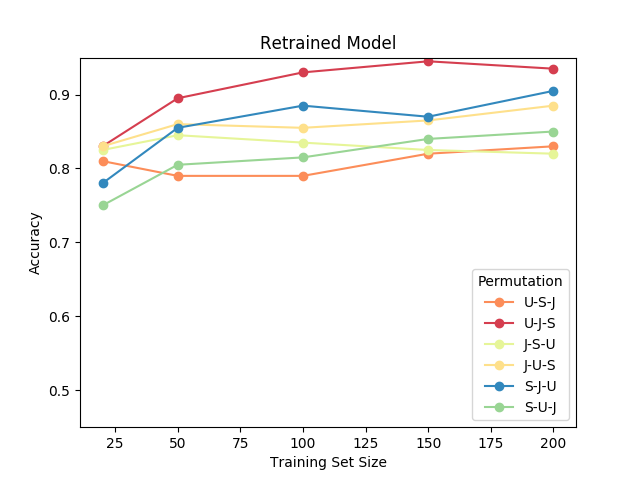
\includegraphics[width=1\textwidth]{images/validation-plot.png}
  \label{fig:validaton-plot}
  \caption{Results of our experiment. As we expected, the graph shows a positive correlation between the accuracy and the number of training samples.}
\end{figure}


\begin{figure}[ht]
  \centering
    \begin{subfigure}{.49\textwidth}
        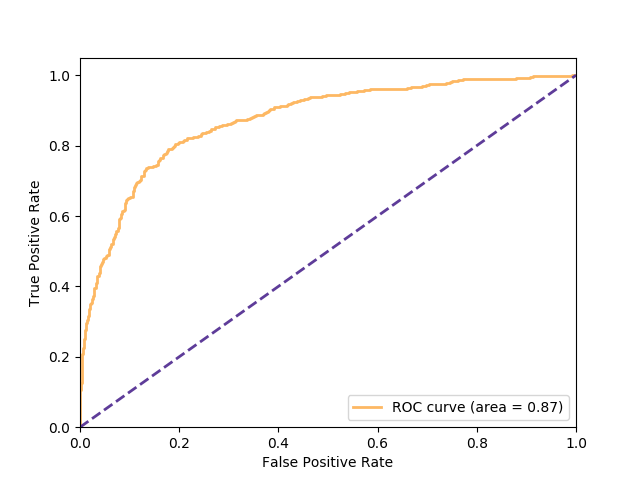
\includegraphics[width=\textwidth]{images/score-10-roc.png}
        \caption{Training Set Size: 20 Images}
    \end{subfigure}
    %
    \begin{subfigure}{.49\textwidth}
        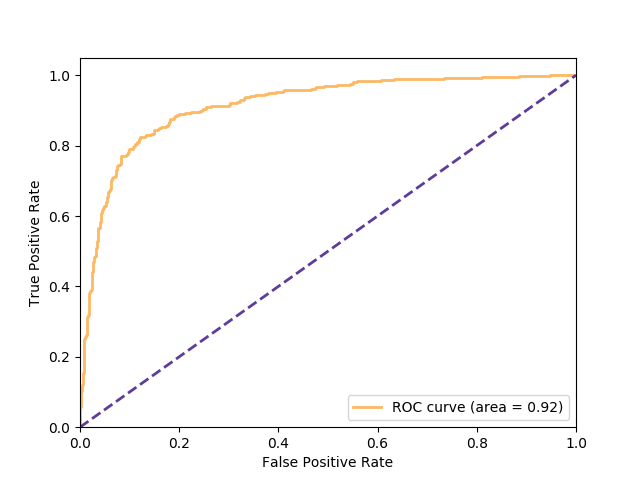
\includegraphics[width=\textwidth]{images/score-25-roc.png}
        \caption{Training Set Size: 50 Images}
    \end{subfigure}
    %
    \begin{subfigure}{.49\textwidth}
        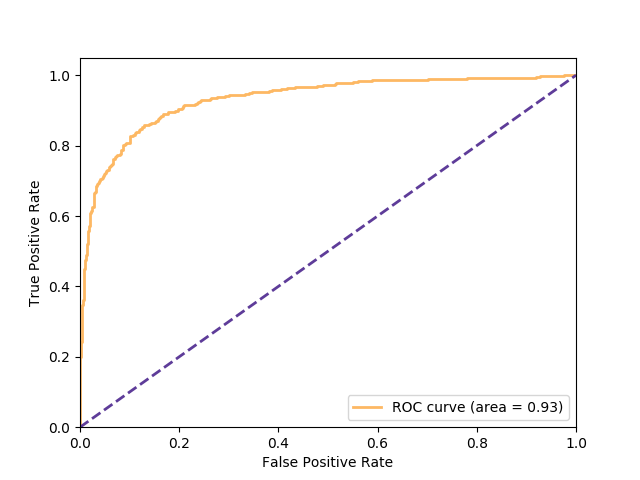
\includegraphics[width=\textwidth]{images/score-50-roc.png}
        \caption{Training Set Size: 100 Images}
    \end{subfigure}
    %
    \begin{subfigure}{.49\textwidth}
        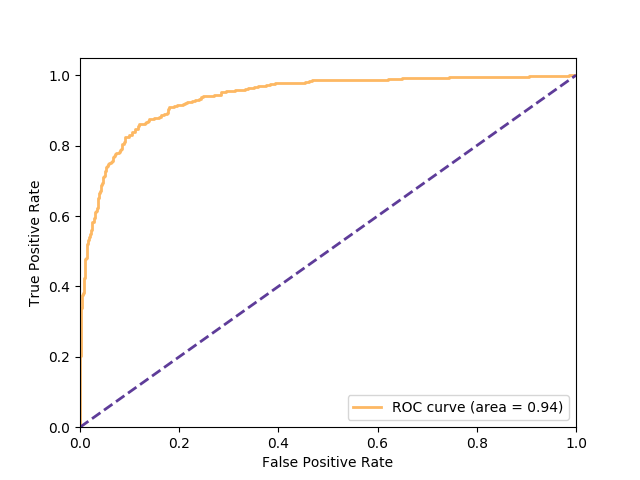
\includegraphics[width=\textwidth]{images/score-75-roc.png}
        \caption{Training Set Size: 150 Images}
    \end{subfigure}
    %
    \begin{subfigure}{.49\textwidth}
        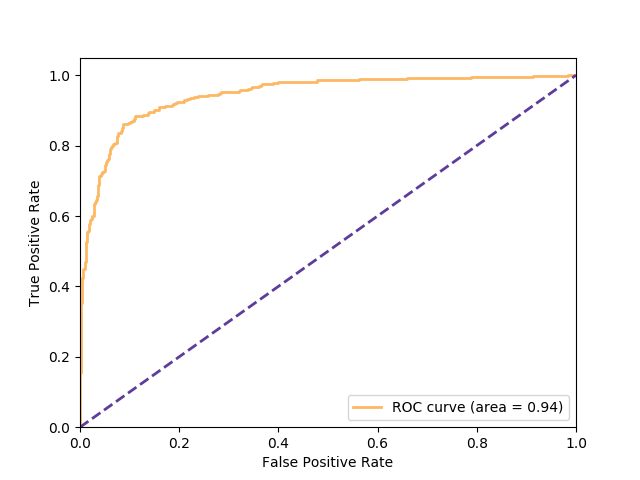
\includegraphics[width=\textwidth]{images/score-100-roc.png}
        \caption{Training Set Size: 200 Images}
    \end{subfigure}
  
  \caption{Receiver operating characteristic curves for the different training sets.}
  \label{fig:whatever}
\end{figure}


\section{Model Validation}

When we train a model, we want it to be a faithful representation of the phenomena that we study, but ¿How do we know that this description is correct? We need to validate the relationship between the outcome of the model and the data that we have at hand. This process is complicated. Validation must be carefully crafted to obtain valid results.\\

One of the difficulties that we found during our research process was that several images might depict the same collapsed building. 
This event could happen when the drone flew over the same territory in different routes. During the tagging stage, we inspected the images for damaged areas, however, despite our efforts, it was impossible to obtain a set of pictures in which every single one was completely independent of the rest. This fact shaped the validation process that we will describe now.\\

Even though deep learning has allowed us to do a giant leap forward on the performance of several tasks, and contrary to what some researchers claim \cite{DBLP:journals/corr/KaiserGSVPJU17}, there exists no universal model. A good model would be able to be performant in very different settings, but it won't be able to handle every situation. We need our model to be robust, but we can not expect it to be perfect. Being aware of the limitations intrinsic to the model is the best way to alleviate possible mistakes. Although it sometimes seems the case, deep learning is not a magic box, it learns from the data that we supply. If the model is biased, in all likelihood, it means that our training set is biased.\\

To have an efficient algorithm, we need it to be performant with places and images it has never seen before. A classic approach would be to divide the dataset into two parts; training and testing sets, the model is trained with the former, and then tested against the latter. This method is not used in practice because data is usually scarce and we would like to take the most of it. A better option is $n-fold$ crossed-validation in which we repeat a similar $n$ times and average the outcomes. This process makes more likely to train the model with every data point and average errors that may appear by chance. However, $n-fold$ crossed-validation does not suit our case because of the nature of the data. Our images were tagged manually; it was the case for some buildings to appear several times in the dataset even though the cropped pictures were not the same. If we apply a technique such as cross-validation, it would be very likely to have the same building both in training and in the testing sets. This situation would lead to having very high accuracies for our model but not such good performance in a real setting. Another thing to be considered is that while traditional supervised classification methods need to divide the dataset into two parts to perform the validation, machine learning methods often require three sets instead, namely train, validation,  and test. The validation test is used during the training stage to select the best performing algorithm, and the testing set is used to see how our model deals with previously unseen data. We manage to elegantly avoid the problem of having repeated data on each of the datasets by using the fact of having information from three completely different settings.\\

To test our model we proposed two different approaches depending on the type of classification involved. With the supervised approaches, images from two towns were used to train the models, and then the remaining one served as test data. In the case of the transfer learning technique, we used one for training, another for validation, and the last one to test the model. We repeated this process in all possible combinations and the accuracies where averaged at the end.\\


\section{How much is enough}


In this section we want to create a benchmark on how much images are needed to perform a retraining of the Inception network. What we wanted to achieve was to demonstrate that it is possible to obtain high accuracys using only a handful of images. We where able to test this by designing an experiment that measures the acurracy of models trained with different sizes of training sets and testing them in a common test set.\\


\section{Threshold selection}

The binary classifier assigns a real number in the interval $[0,1]$. To decide which values will be assigined with either level a threshold must be chosen. This was picked using a ROC curve. The ROC curve helps us chosing the performance that fits our needs in the ver possible way. In order to do this we use a receiver operating characteristic curve. This tool is often used with binary classifiers to analyse the tradeoff between the true possitive rate and the false possitive rate by selecting different desicion thresholds.\\

The threshold was chosen to keep the false positive rate to 0 percent on the training set while having the highest level of true positive rate. This was atained at the following level.\\

The reason behind this decision was the high number of false positives shown in preliminary experiments. We want only to look at places in which the model is very confident of finding a damaged building. This theshold can be tunned to match the desired behavior in the requiered application.\\

\section{Results}

Ortorectified mosaics where built by CENAPRED using the very same images taht we used to train our models. This images come in a different format than the images taken by the drones. Additional to the optical information these tif files contain geographical location and can be used to assing a point in space to each pixel in the image. This means that we can not only locate a damaged building in an image, but to link this information with a geographical location in a given projection.\\

The images where divided in a regular grid of 299 pixel tiles with 90 pixel ovelaps. These overlaps are later postprocessed to eliminate the posibility of counting the same building twice. Each tile is exposed to the model which predicts a class on it using the previously selected threshold. When the model test a tile positive, the box is saved for postprocesing in which a technique known as non max suppression is used to eliminate boxes that represent the same object. This technique is borrowed from facial recognition algorithms. Once we have the final boxes, the center pixel of each box is transformed to world coordinates. Additionaly, this coordinates are used to query Google Maps API to obtain a human readable address for each point.\\

A shape file is produced which contains the results for each town given the output of the algorithm. This shape can be overlayed on top of the raster file using a Geographic Information System software such as QGIS. Additionaly the results are also exposed via the REST interface so they can be visualised in the web application.\\













\begin{center}
  \begin{tabular}{|c|c|c|c|c|c|}
    \hline
         &20 Images &50 Images &100 Images&150 Images&200 Images\\ \hline
    U-S-J&0.55      &0.66      &0.77      &0.84      &0.81      \\ \hline
    U-J-S&0.9       &0.94      &0.93      &0.92      &0.94      \\ \hline
    J-S-U&0.65      &0.78      &0.77      &0.82      &0.78      \\ \hline
    J-U-S&0.8       &0.82      &0.85      &0.847     &0.895     \\ \hline
    S-J-U&0.7       &0.78      &0.86      &0.9       &0.895     \\ \hline
    S-U-J&0.75      &0.72      &0.83      &0.833     &0.86      \\
     
    \hline
  \end{tabular}
\end{center}





\begin{center}
  \begin{tabular}{|c|c|c|}
    \hline
    threshold & true positive rate & false positive rate \\ \hline
    0.983629 & 0.529412 & 0.0 \\
    \hline
  \end{tabular}
\end{center}




\begin{center}
  \begin{tabular}{|c|c|c|c|c|c|}
    \hline
    town                 & positives & width & height & time (seconds) & overlap\\ \hline
    Santa Maria Xadani   &51         & 25598 & 30144  & 4420           & 0.1 \\ \hline
    Juchitan de Zaragoza &302        & 42375 & 28831  & 6375           & 0.1 \\ \hline
    Union Hidalgo        &25         & 19945 & 28795  & 3938           & 0.1\\
    \hline
  \end{tabular}
\end{center}




